\documentclass[12pt,a4paper]{report}

%====================== PACKAGES ======================

\usepackage[french]{babel}
\usepackage[utf8x]{inputenc}
%pour gérer les positionnement d'images
\usepackage{float}
\usepackage{amsmath}
\usepackage{graphicx}
\usepackage[colorinlistoftodos]{todonotes}
\usepackage{url}
%pour les informations sur un document compilé en PDF et les liens externes / internes
\usepackage{hyperref}
%pour la mise en page des tableaux
\usepackage{array}
\usepackage{tabularx}
%pour utiliser \floatbarrier
%\usepackage{placeins}
%\usepackage{floatrow}
%espacement entre les lignes
\usepackage{setspace}
%modifier la mise en page de l'abstract
\usepackage{abstract}
%police et mise en page (marges) du document
\usepackage[T1]{fontenc}
\usepackage[top=2cm, bottom=2cm, left=2cm, right=2cm]{geometry}
%Pour les galerie d'images
\usepackage{subfig}

%====================== INFORMATION ET REGLES ======================

%rajouter les numérotation pour les \paragraphe et \subparagraphe
\setcounter{secnumdepth}{4}
\setcounter{tocdepth}{4}
\makeatletter
\hypersetup{							% Information sur le document
pdfauthor = {Premier Auteur,
			Deuxième Auteur,
			Troisième Auteur,
    		Quatrième Auteur},			% Auteurs
pdftitle = {Nom du Projet -
			Sujet du Projet},			% Titre du document
pdfsubject = {Mémoire de Projet},		% Sujet
pdfkeywords = {Tag1, Tag2, Tag3, ...},	% Mots-clefs
pdfstartview={FitH}, 					% Ajuste la page à la largueur de l'écran
colorlinks = true, 						% Colorise les liens
breaklinks = true, 						% Permet le retour à la ligne dans les liens trop longs
urlcolor = blue, 						% Couleur des hyperliens
linkcolor = blue, 						% Couleur des liens internes
citecolor = blue,    						% Couleur des liens de citations
bookmarksopen = true,
pdftoolbar = false,
pdfmenubar = false
}					
%pdfcreator = {MikTeX},% Logiciel qui a crée le document
%pdfproducer = {}} % Société avec produit le logiciel

%======================== DEBUT DU DOCUMENT ========================

\begin{document}

%régler l'espacement entre les lignes
\newcommand{\HRule}{\rule{\linewidth}{0.5mm}}

%page de garde

\begin{titlepage}
    \begin{center}
    
    % Upper part of the page. The '~' is needed because only works if a paragraph has started.
    
    \begin{tabular}{cc}
  
\includegraphics[width=0.4\textwidth]{./img/ua_h_couleur}
  \hspace{4cm}
    
\includegraphics[width=0.4\textwidth]{./img/Dpt_Info}
	\end{tabular}    
    
      \vspace{1cm}

	
	
\includegraphics[width=0.4\textwidth]{./img/irset}~\\[1cm]

    
    \textsc{\Large }\\[0.5cm]
    
    % Title
    \HRule \\[0.4cm]
    
    {\huge \bfseries Concrétisation disciplinaire\\
   Projet ESTER \\[0.4cm] }
    
    \HRule \\[1.5cm]
    
    % Author and supervisor
    \begin{minipage}{0.4\textwidth}
    \begin{flushleft} \large
    
     \emph{ESTER:}\\
    Natacha \textsc{Fouquet}\\
    Anna \textsc{Lloyd}\\
    \textsc{\Large }\\[0.3cm]
    \emph{Référents:}\\
    Vincent \textsc{Barichard}\\
    Laurent \textsc{Garcia}
    David \textsc{Genest}
    Jean-Michel \textsc{Richer}
    
    \end{flushleft}
    \end{minipage}
    \begin{minipage}{0.4\textwidth}
    \begin{flushright} \large
    
	\emph{Chefs de projet (M2):}\\
    Hugues \textsc{Dumont}\\
    Guillaume \textsc{Huet}\\
    Zineb \textsc{Loukili}\\
    \textsc{\Large }\\[0.3cm]
    \emph{Équipe de développement (M1):}\\
    Nidal \textsc{Bedyouch}\\
    Imane \textsc{Belhouari}\\
    Théo \textsc{Dézé}\\
    Charles \textsc{Mallet}    
    \end{flushright}
    \end{minipage}
    
    \vfill
    
    % Bottom of the page
    {\large \today}
    
    \end{center}
    \end{titlepage}

%page blanche
\newpage
~
%ne pas numéroter cette page
\thispagestyle{empty}
\newpage

%\input{./abstract.tex}

\tableofcontents
\thispagestyle{empty}
\setcounter{page}{0}
%ne pas numéroter le sommaire

\newpage

%espacement entre les lignes d'un tableau
\renewcommand{\arraystretch}{1.5}

%====================== INCLUSION DES PARTIES ======================

~
\thispagestyle{empty}
%recommencer la numérotation des pages à "1"
\setcounter{page}{0}
\newpage

%\input{./presentation.tex}

%\input{./existant.tex}
 
%\input{./besoins.tex}

%\input{./autre_partie.tex}

\chapter{Partie Théo Dézé}

\section{Base de Données}

La base de données est divisée en plusieurs collections.

Pour l'implémentation, nous avons utilisé le driver officiel proposer par MongoDB pour le Java. Nous avons crée une classe mère en Java utilisée par héritage et qui permet de définir des interfaces simplifiant l'utilisation du reste du code.

\subsection{Utilisateur ESTER}

\begin{figure}[H]
    \begin{center}
        \begin{tabularx}{17cm}{|c|X|}
            \hline
            Clé & Valeur  \tabularnewline 
            \hline
            Identifiant & 
            Chaine de caratères, peut être utilisé à la place du mail lors de la connexion \tabularnewline 
            Nom & 
            Chaine de caratères \tabularnewline
            Prénom & 
            Chaine de caratères \tabularnewline
            Première connexion & 
            Boolean \tabularnewline
            Mot de passe & 
            Chaine de caratères chiffrée \tabularnewline
            Mail & 
            Chaine de caratères \tabularnewline
            Statut & 
            Chaine de caratères, représente le statut de l'Utilisateur (Médecin, Administrateur,
            Préventeur, Assistant) \tabularnewline
            \hline
        \end{tabularx}
    \end{center}
    \caption{Tableau de la collection Utilisateur}
\end{figure}

La collection correpond à celle prévue par nos chefs de projet comme
les collections Entreprise et Salarie qui sont des collections proches (L'entreprise ne possède 
pas d'email et le salarie n'a pas de mots de passe mais a la liste des questionnaires répondus ou à répondre
) de Utilisateur ESTER donc nous ne nous répéterons pas. 


\subsection{Questionnaire}

\begin{figure}[H]
    \begin{center}
        \begin{tabularx}{17cm}{|c|X|}
            \hline
            Clé & Valeur  \tabularnewline 
            \hline
            Nom & 
            Nom du questionnaire \tabularnewline 
            Identifiant & 
            Version simplifiée du nom \tabularnewline
            Identifiant ESTER & 
            Identifiant de la personne qui a soumis le questionnaire \tabularnewline
            Date de soumission & 
            Date \tabularnewline
            Mail & 
            Chaine de caratères \tabularnewline
            HTML & 
            Chaine de caratères (HTML brut) \tabularnewline
            \hline
        \end{tabularx}
    \end{center}
    \caption{Tableau de la collection Questionnaire}
\end{figure}

\subsection{Réponse}

\begin{figure}[H]
    \begin{center}
        \begin{tabularx}{17cm}{|c|X|}
            \hline
            Clé & Valeur  \tabularnewline 
            \hline
            Identifiant salarie & 
            Identifiant du salarie qui a répondu \tabularnewline
            Identifiant questionnaire & 
            Identifiant du questionnaire répondu \tabularnewline
            Reponses & 
            Tableau associatif qui lie les identifiants des réponses 
            avec leurs réponses \tabularnewline
            \hline
        \end{tabularx}
    \end{center}
    \caption{Tableau de la colection Réponse}
\end{figure}
\subsection{Sécurité}

Nous stockons des mots de passe dans la base de données, nous avons eu besoin de sécuriser les mots de passe pour ne pas les stocker en clair.
Nous avons comparé plusieurs technologies MD5, SHA256, SHA512, PBKDF2, BCrypt et SCrypt. Ce sont tous des fonctions de hachage mais certaines proposent des bases de salage (PBKDF2, BCrypt, SCrypt) qui permettent de se protéger contre les attaques utilisant des rainbows tables ou par dictionnaire. 
Certaines fonctions de hachage sont difficilement optimisables ce qui permet de rendre plus difficile les attaques par la force brute. De ce fait, cela donne le temps à l'utilisateur de changer sont mot de passe.     

Nous avons choisi d'utilisé BCrypt car il propose une implémentation en java et il fait partie des algorithme les plus sécurisés.
\section{Connexion}

\subsection{Génération chaîne de caractère aléatoire}
    
\begin{itemize} 
\item Problématique :
Lors de la création d’un utilisateur ESTER par un autre (un médecin peut créer un compte infirmier, assistant, préventeur, et un administrateur peut tout créer), un mot de passe provisoire est communiqué à l’utilisateur pour sa première connexion.
D’autre part, le patient se connecte en utilisant un identifiant unique de 5 caractères communiqué par son médecin.
\item  Implémentation :
Pour l’implémentation, nous avons utilisé une instance de la classe SecureRandom \footnote{Cette classe fournit un générateur de nombres aléatoires (RNG) de chiffrement fort.} permettant de tirer aléatoirement les caractères de la chaîne et de la permuter aléatoirement afin d’être imprédictible.
\item  Bilan :
Le générateur de chaîne de caractères aléatoires est fonctionnel et sera utilisé pour la génération de mot de passe provisoire. Tandis que, l’identifiant du patient sera abandonné vu que la complexité de vérification de l’unicité est haute. Les M2 se chargeront de définir un algorithme générant des identifiants cryptés et uniques.

\end{itemize}

\begin{figure}[H]
    \begin{center}
	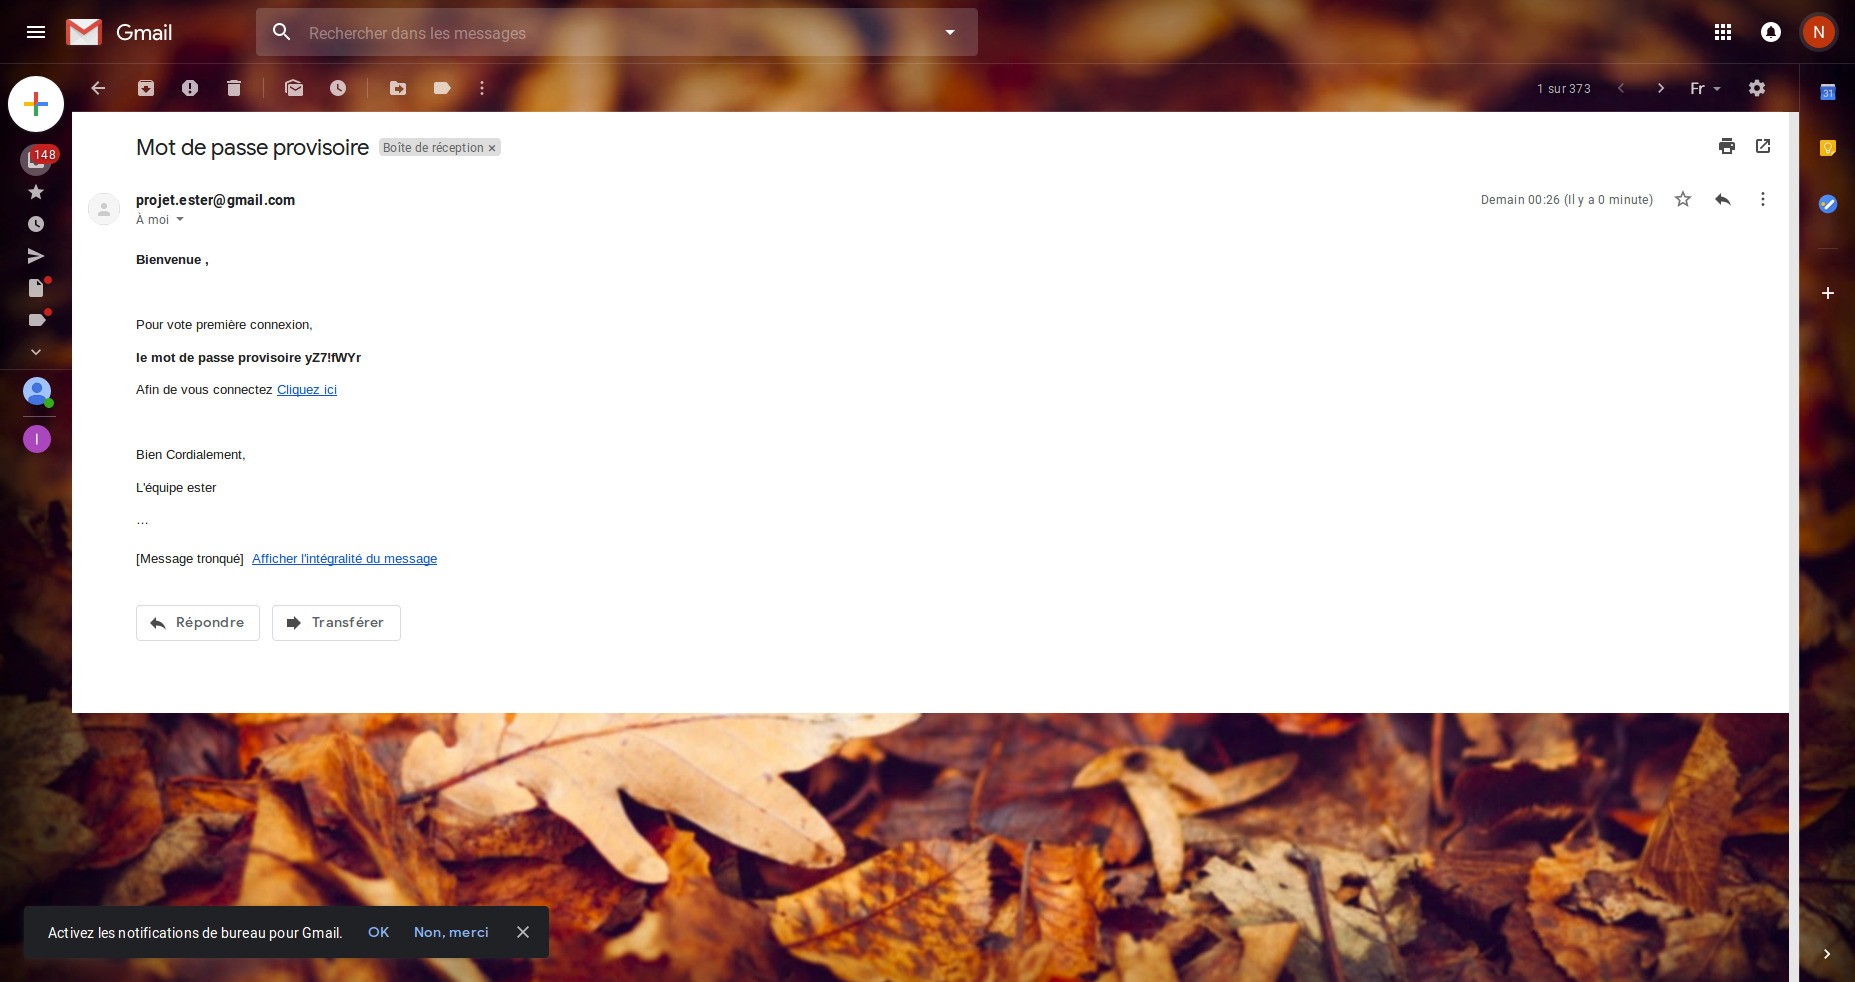
\includegraphics[scale=0.25]{img/connexion/mailCo}
    \end{center}
    \caption{E-mail pour la première connexion}
\end{figure}

\begin{figure}[H]
    \begin{center}
	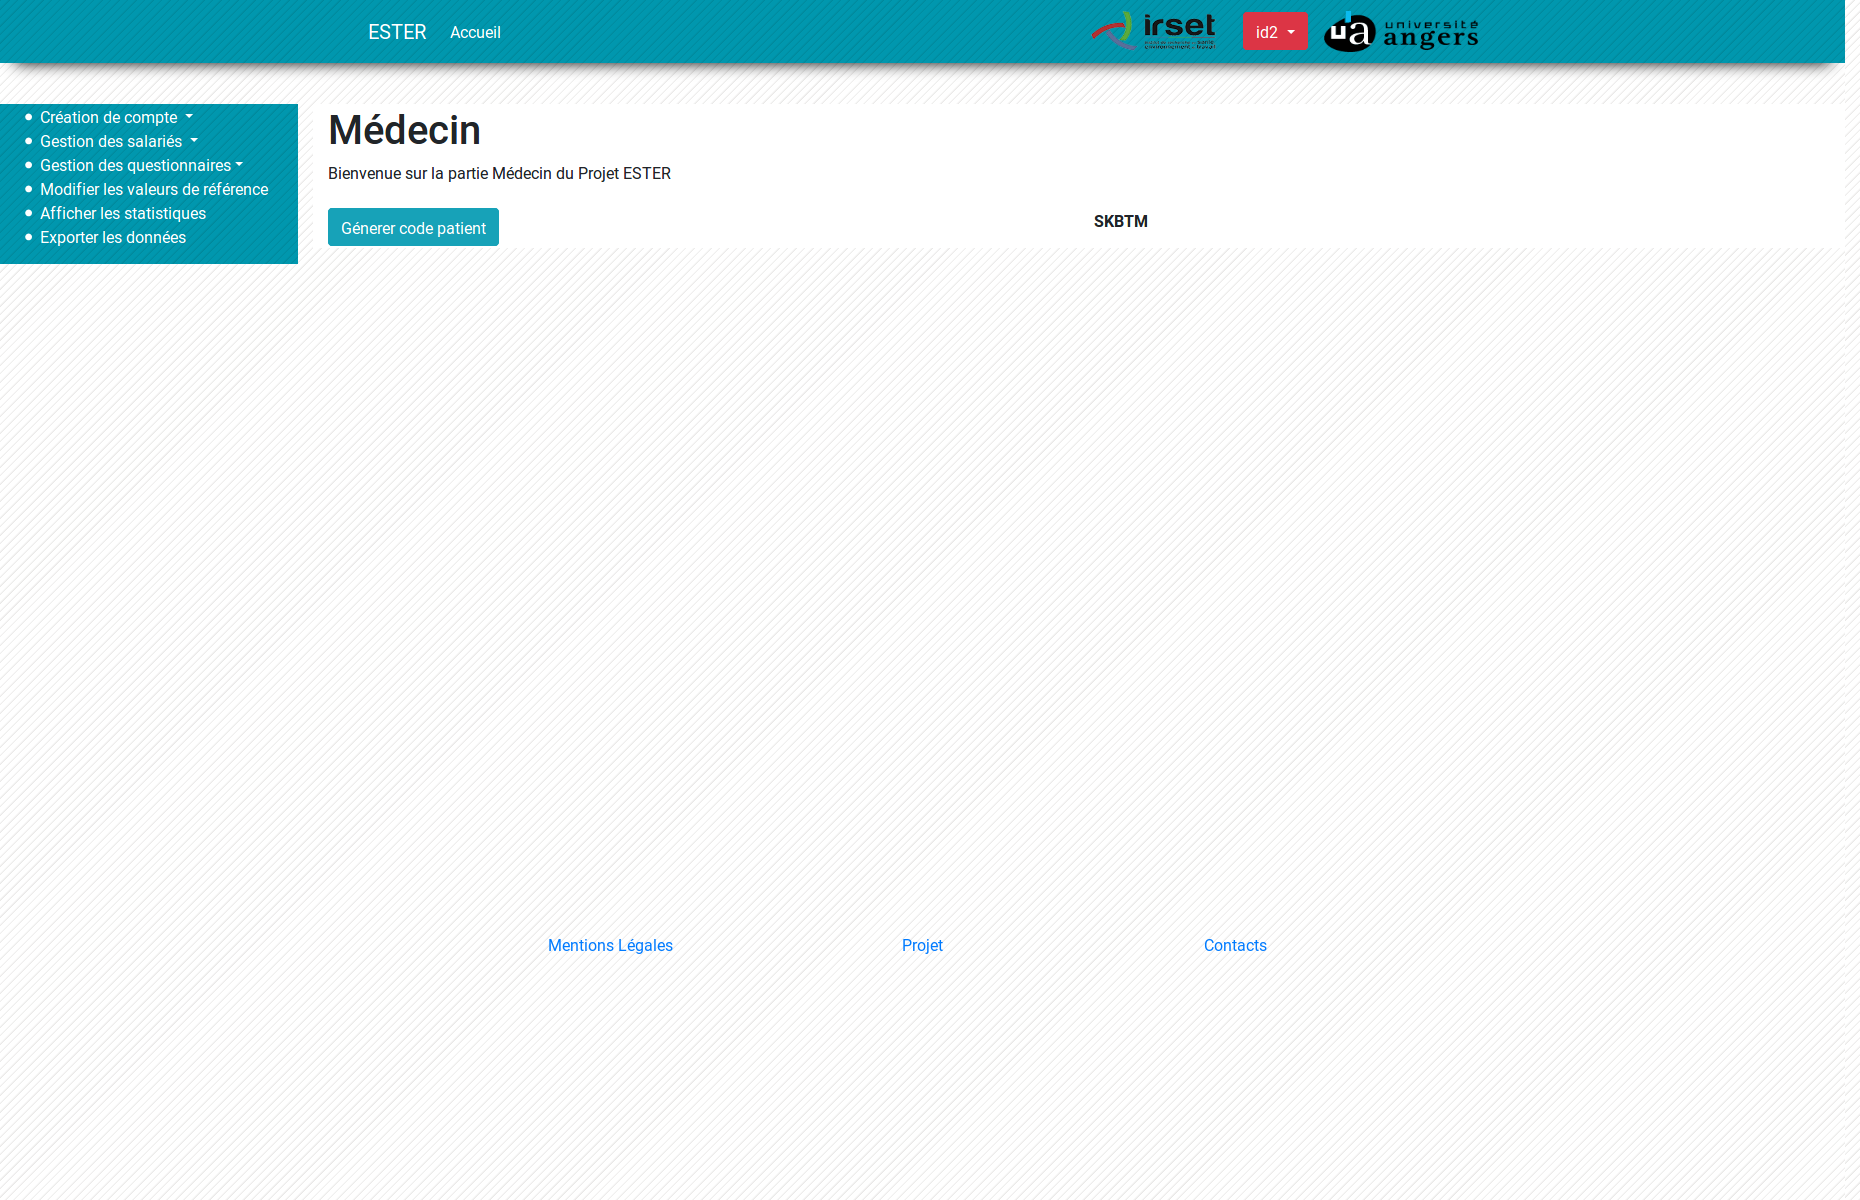
\includegraphics[scale=0.25]{img/connexion/medecin}
    \end{center}
    \caption{Générateur de codes patients}
\end{figure}

\subsection{Formulaire première connexion patient}

Lors de la création d’un compte patient seul l’identifiant est enregistré en base de données. Et afin de compléter les informations manquantes au profil à titre d'illustration: le sexe, l’âge quinquennal (pour préserver l’anonymat du patient), poste de travail, secteur d’activité et département, le patient est redirigé lors de sa première connexion vers le formulaire ci-dessous.

\begin{figure}[H]
    \begin{center}
	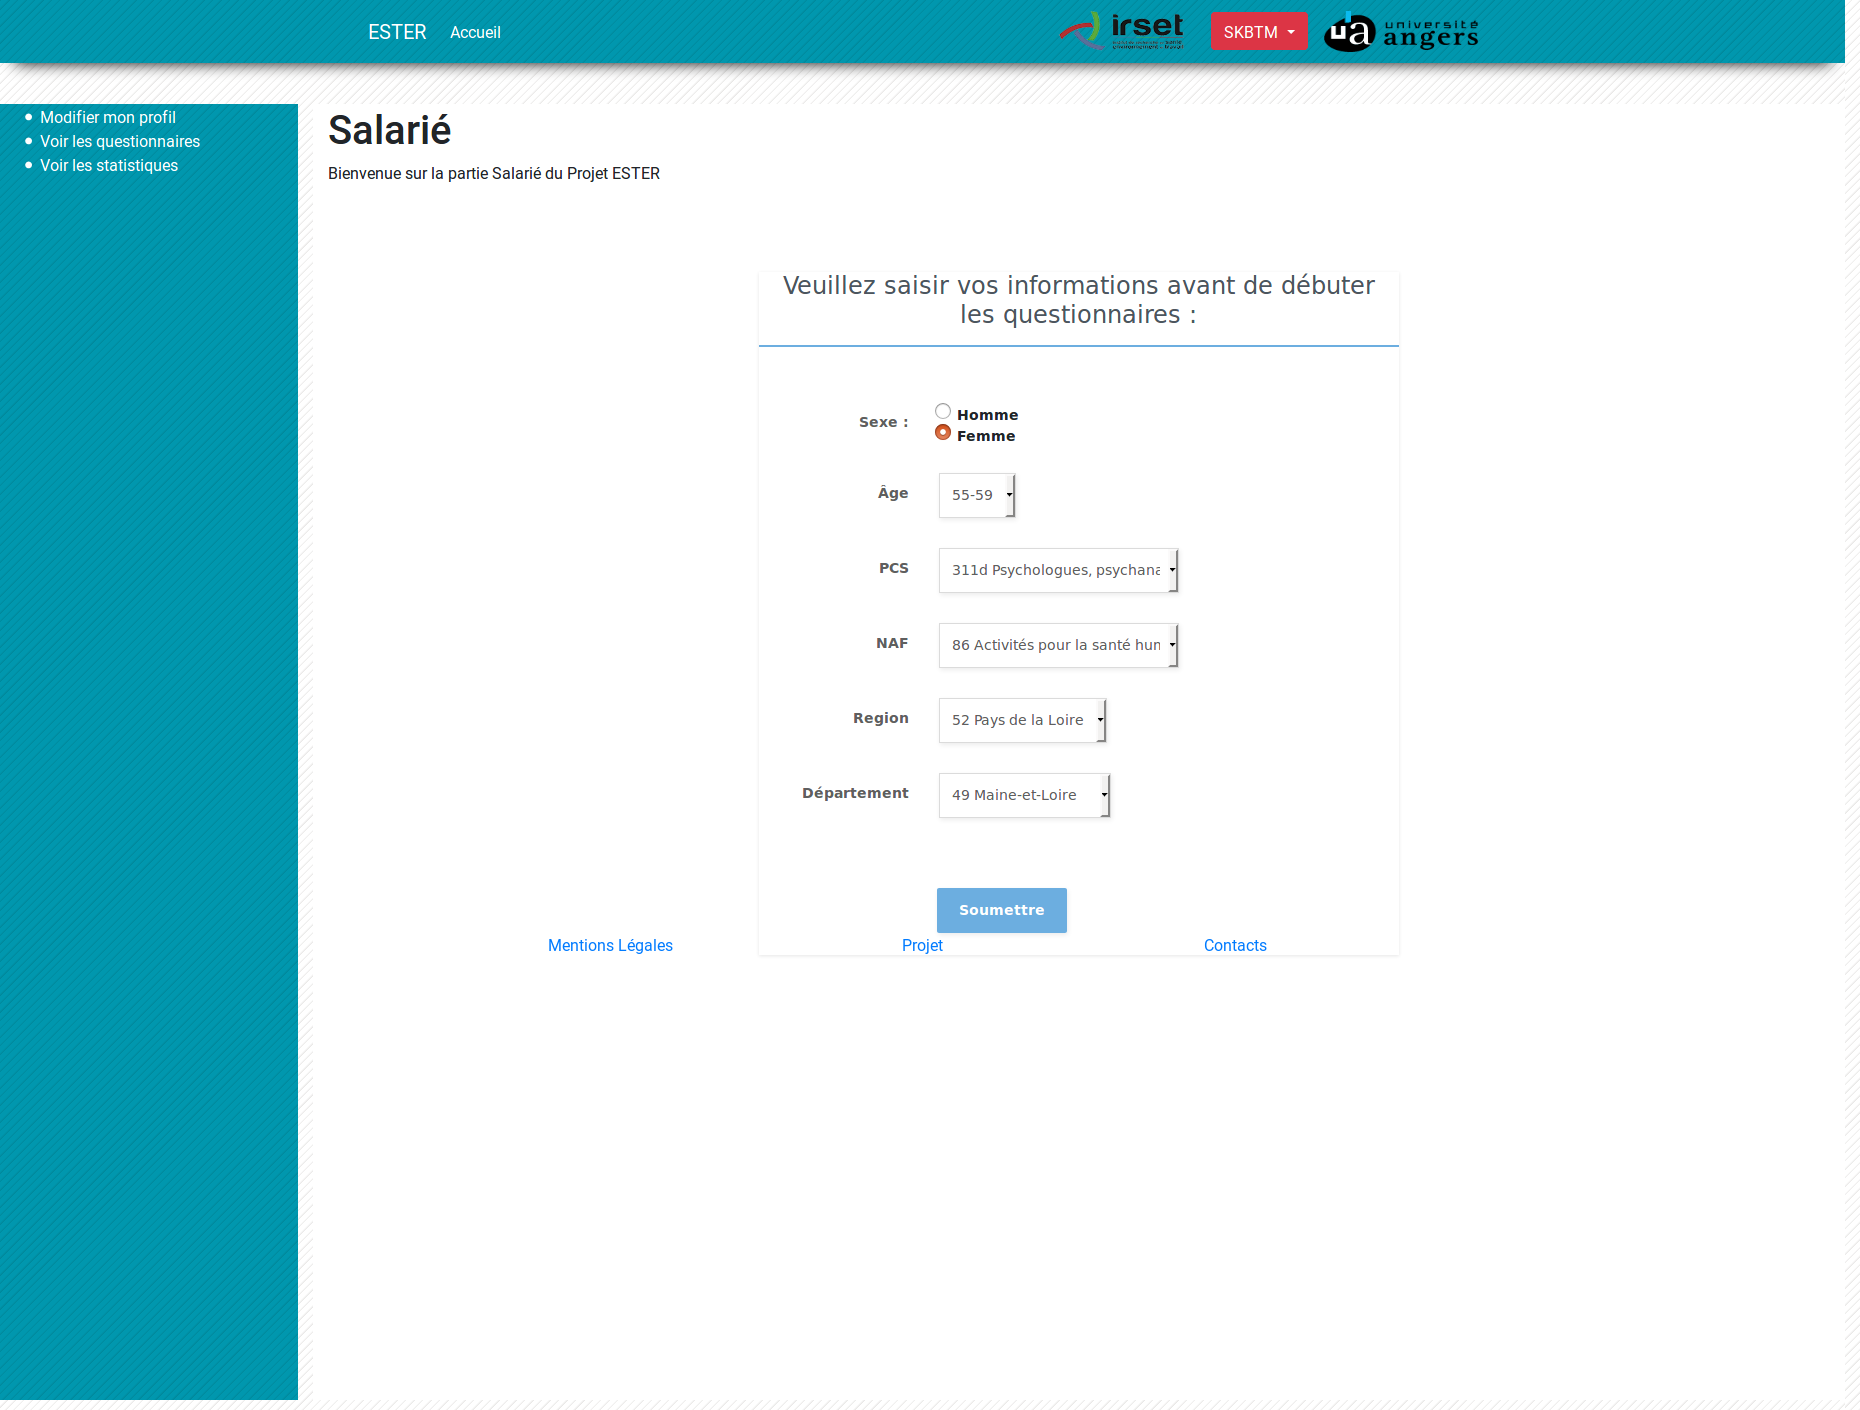
\includegraphics[scale=0.25]{img/connexion/formPatient}
    \end{center}
    \caption{Formulaire du patient à la première connexion}
\end{figure}

\section{Résultat}

\subsection{Choix}

\subsubsection{Besoin}

Le projet, nous demande une certaine mise en forme (voir figure si dessous) des résultats. Dans les besoins, il avais aussi d'exporter les donnée dans diverses formats CSV, PDF, PNG et autres et d'être compatible avec les PC/Tablette/Smartphone.  

\begin{figure}[H]
    \begin{center}
    
\includegraphics[height=2.0cm]{img/mongodb}
    \end{center}
    \caption{Mise en forme des résultat demandé}
\end{figure}

\subsubsection{Highcharts}

Highcharts est un librairie JavaScript qui permet de généré des graphiques interactifs. Les paramétrages s'effectue en JSON et offre la possibilité export dans les différents formats.

\begin{figure}[H]
    \begin{center}
    
\includegraphics[height=2.0cm]{img/mongodb}
    \end{center}
    \caption{Logo de Highcharts}
\end{figure}

\subsection{Implémentation}

\subsubsection{Highcharts}

L'implémentation de base de Highcharts a été assez simple, mais la création des lignes de séparation (exemple "D'accord vs Pas d'accord") et de coche pour les réponses du le salarie on demandé plus de temps. 

Ce temps en plus est du au temps à la nécessité pour l'adapter a nos besoins. Car certaine n'avais pas des fonctions par défaut pour efféctuer les taches si dessus.

\subsubsection{DWR}

DWR (Direct Web Remoting) est un librairie Java qui permet de recevoir des résultats du serveur sur le principe Ajax (asynchronous JavaScript and XML) qui permet de faire des requêtes aux serveur, mais de manière simplifier.

Cette librairie nous permet de faire le line entre Highcharts et notre serveur pour récupéré les information telle que les questions et leurs valeurs (réponse et pourcentage).

\subsection{Bilan}

Le rendus des résultat est fonctionnel 

\begin{figure}[H]
    \begin{center}
    
\includegraphics[height=2.0cm]{img/mongodb}
    \end{center}
    \caption{Mise en forme des résultat rendus final}
\end{figure}

%\input{./bilan.tex}

%\input{./annexes.tex}

\newpage

%récupérer les citation avec "/footnotemark"
\nocite{*}

%choix du style de la biblio
\bibliographystyle{plain}
%inclusion de la biblio
\bibliography{bibliographie.bib}
%voir wiki pour plus d'information sur la syntaxe des entrées d'une bibliographie

\end{document}